\documentclass{article}

\usepackage{graphicx}
\usepackage{float}
\usepackage{amssymb}

\title{Machine Intelligence 2 - Exercise 5\\
Principle component analysis and whitening}
\author{Jens Krenzin - 319308\\
Till Rohrmann - 343756}
\date{\today}

\begin{document}
	\maketitle
	\setcounter{section}{4}
	\subsection{Preprocessing}
		The given dataset is plotted in Figure \ref{fig:task1Input}. Additionally the calculated principle components, green from the whole dataset and red excluding the outliers, are shown.
		\begin{figure}[H]
			\centering
			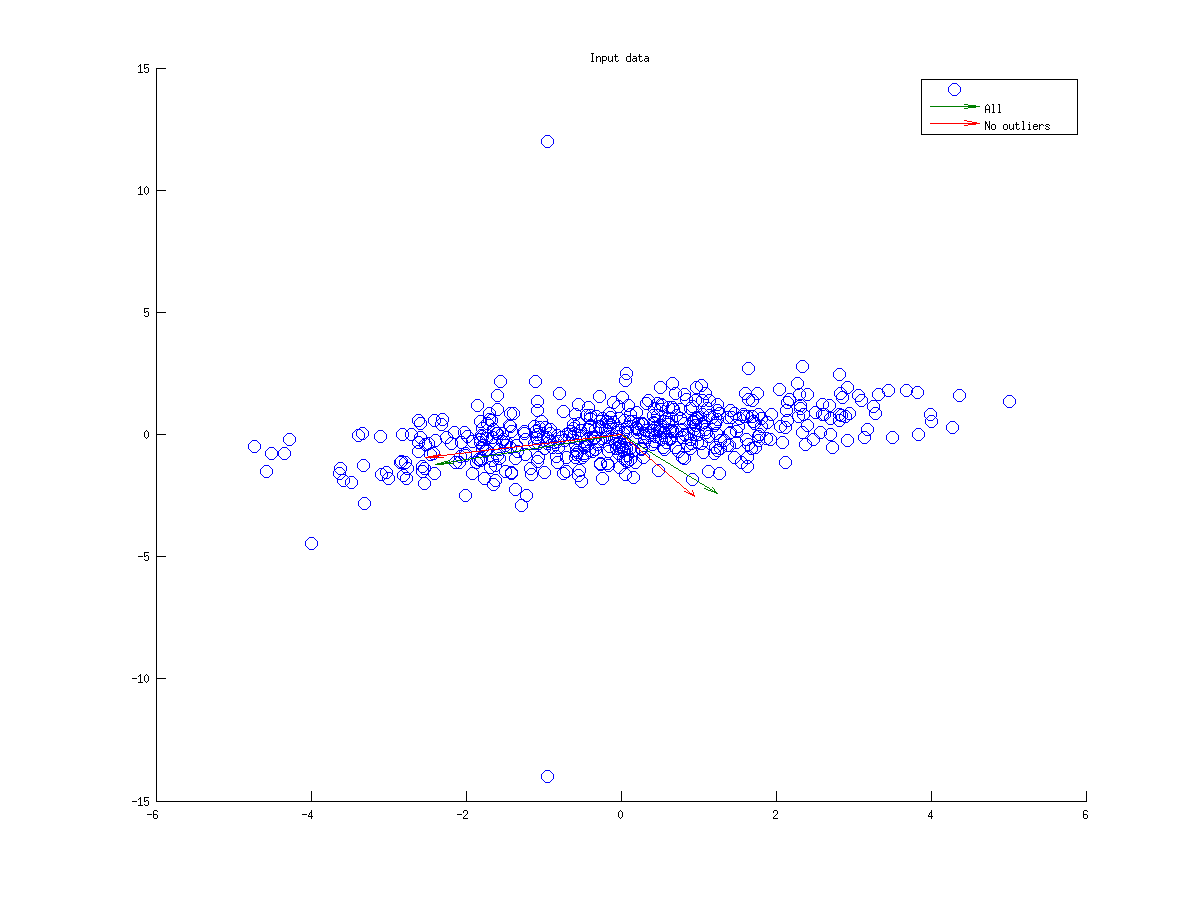
\includegraphics[width=10cm]{task1Input.png}
			\caption{Centralized input data}
			\label{fig:task1Input}
		\end{figure}
		
		We can see in Figure \ref{fig:task1Projection} that there are two datapoints which are clear outliers. They coarsen the y-scale unnecessarily.
		\begin{figure}[H]
			\centering
			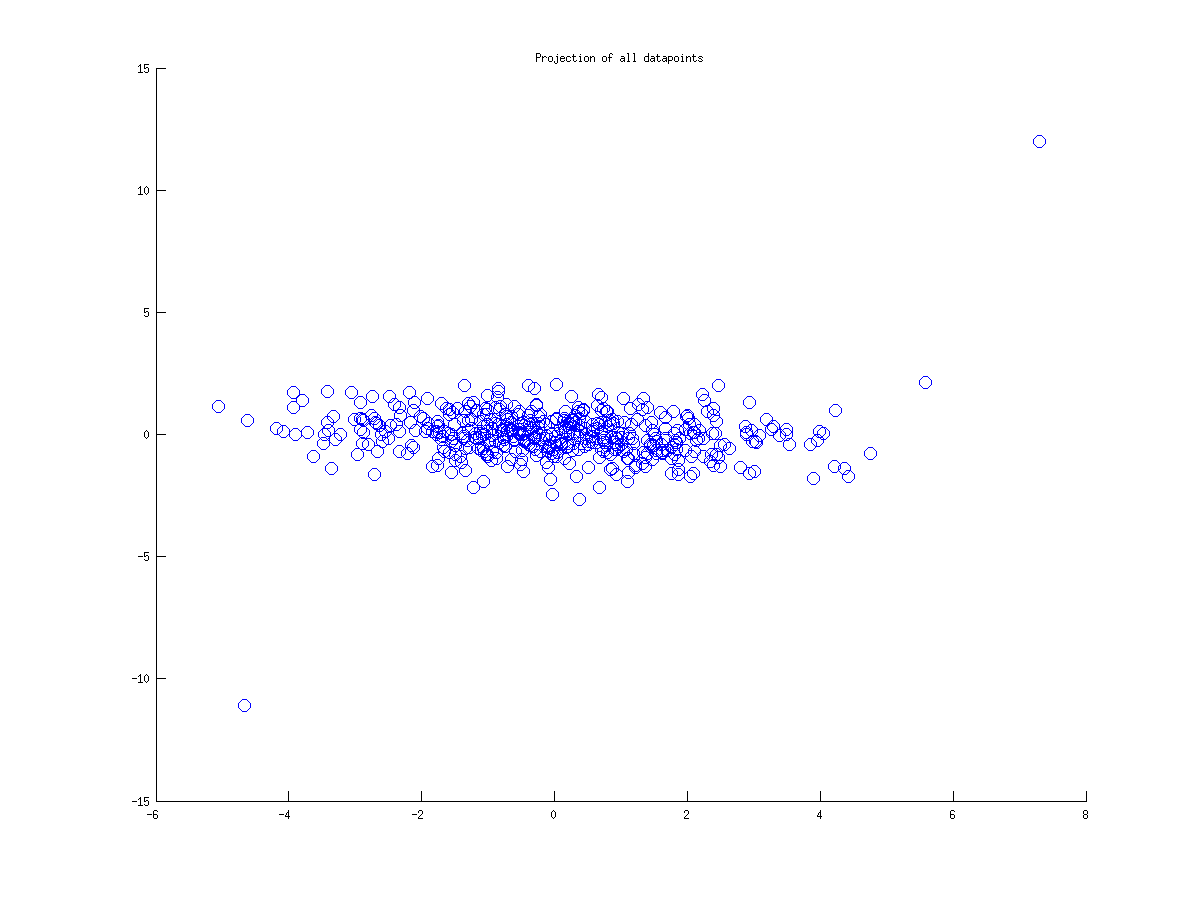
\includegraphics[width=10cm]{task1Projection.png}
			\caption{Projection according to PCs of complete dataset}
			\label{fig:task1Projection}
		\end{figure}
		
		Removing the outliers produces considerably different principle components as it can be seen in Figure \ref{fig:task1Input}. The result of the projection can be seen in \ref{fig:task1ProjectionWithoutOutliers}
		\begin{figure}[H]
			\centering
			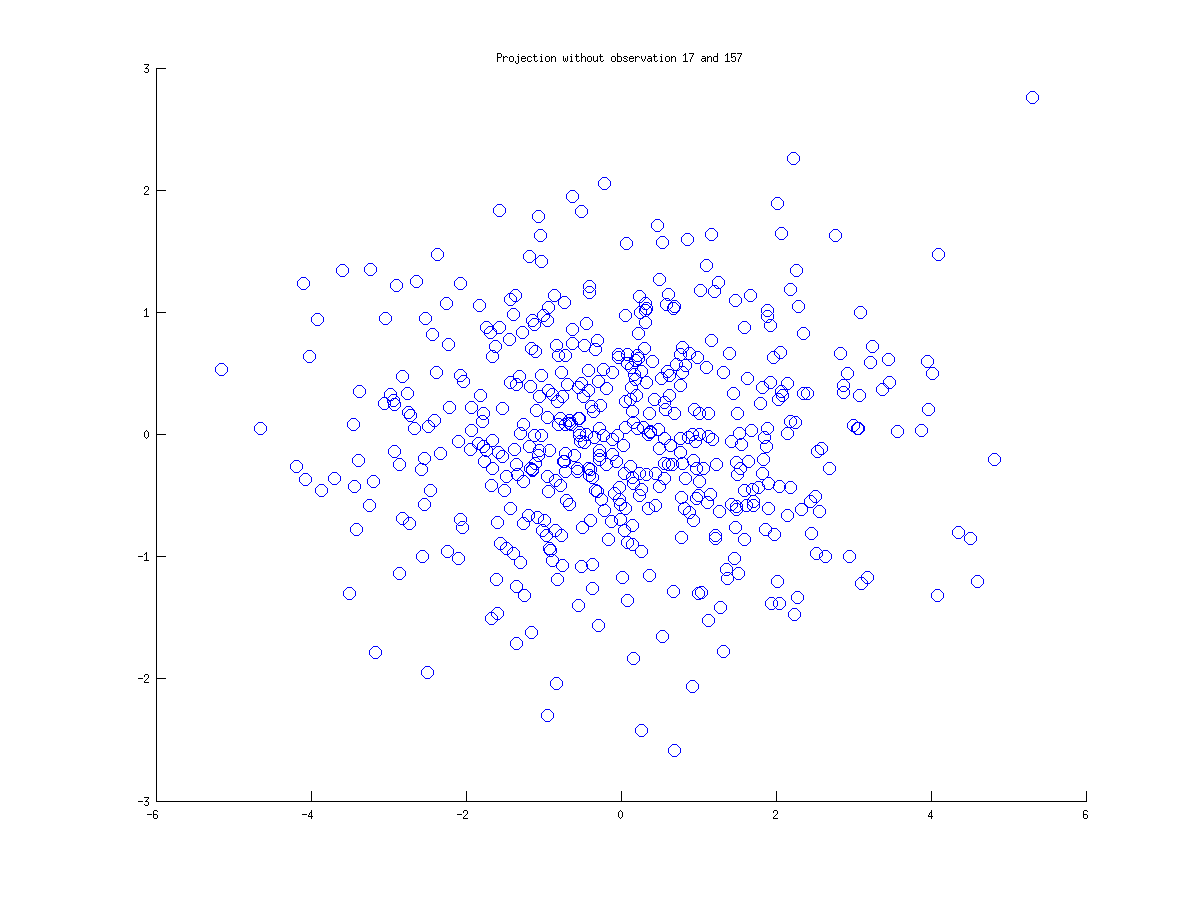
\includegraphics[width=10cm]{task1ProjectionWithoutOutliers.png}
			\caption{Projection according to PCs of dataset excluding the outliers}
			\label{fig:task1ProjectionWithoutOutliers}
		\end{figure}
	\subsection{Whitening}
		We have checked the data for outliers using the Chauvenet's criterion. 
		It assumes the data to be normally distributed and then checks the probability of their occurrence. 
		If the probability of its occurrence is $<0.5$ then the point is discarded.
		This method found $5$ outliers and is done as a preprocessing step.
		The following scree plot is shown in Figure \ref{fig:task2ScreePlot}.
		\begin{figure}[H]
			\centering
			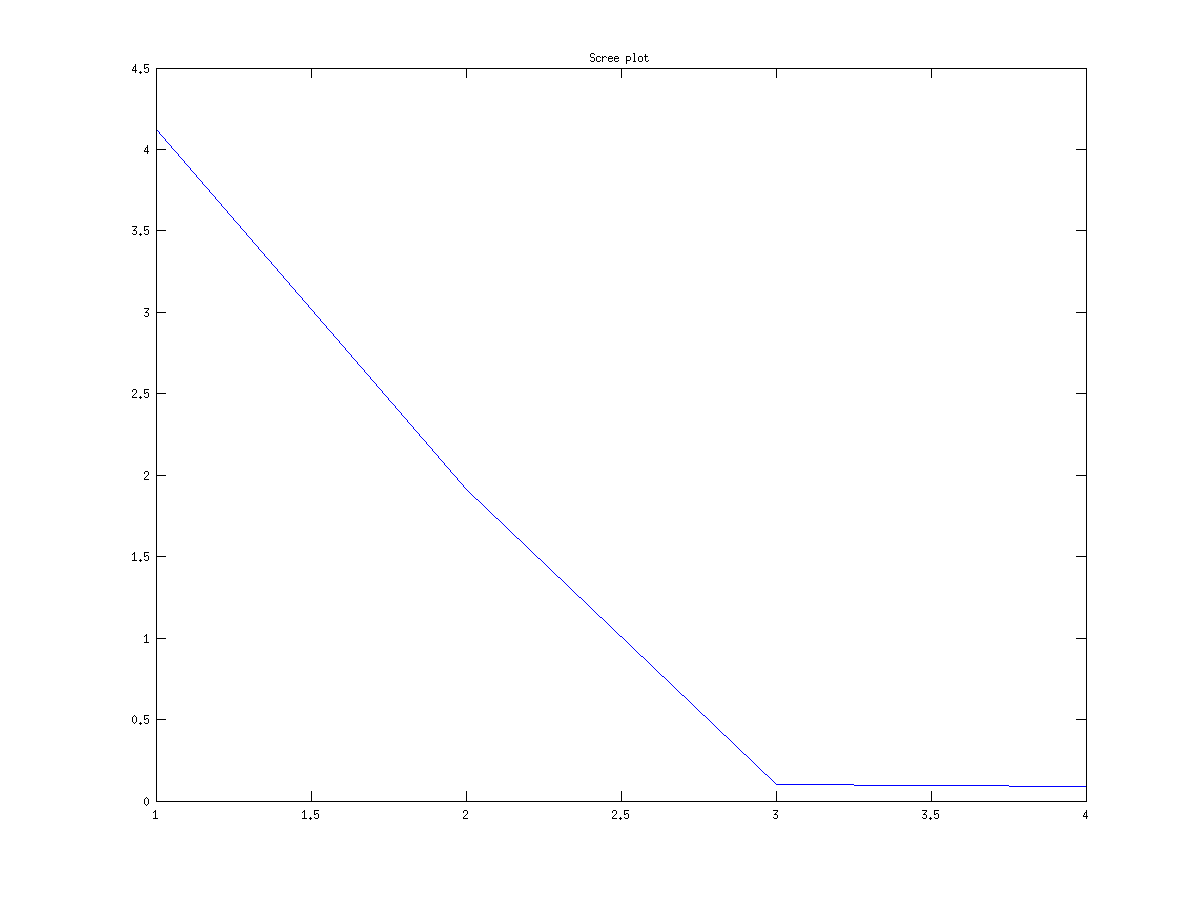
\includegraphics[width=10cm]{task2ScreePlot.png}
			\caption{Scree plot}
			\label{fig:task2ScreePlot}
		\end{figure}
		As we can see, we only need the principle components corresponding to the two biggest eigenvalues to represent the data sufficiently.
		
		The covariance matrix of the filtered input data is given in Figure \ref{fig:task2Covariance}. 
		The covariance of the projected data is given in Figure \ref{fig:task2Eigenvalues} and the whitened data is shown in Figure \ref{fig:task2WhitenedData}.
		
		\begin{figure}[H]
			\centering
			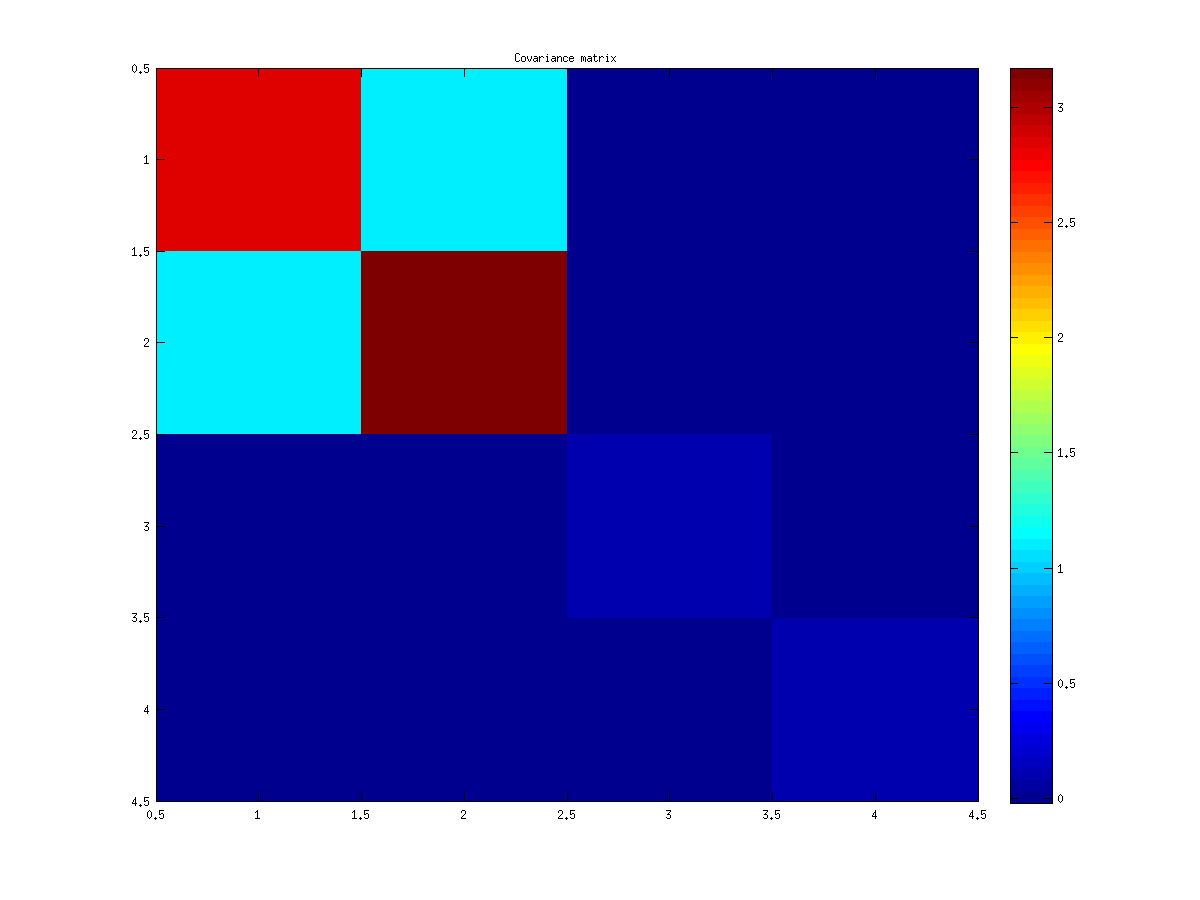
\includegraphics[width=10cm]{task2Covariance.png}
			\caption{Covariance matrix of input data}
			\label{fig:task2Covariance}
		\end{figure}
		
		
		\begin{figure}[H]
			\centering
			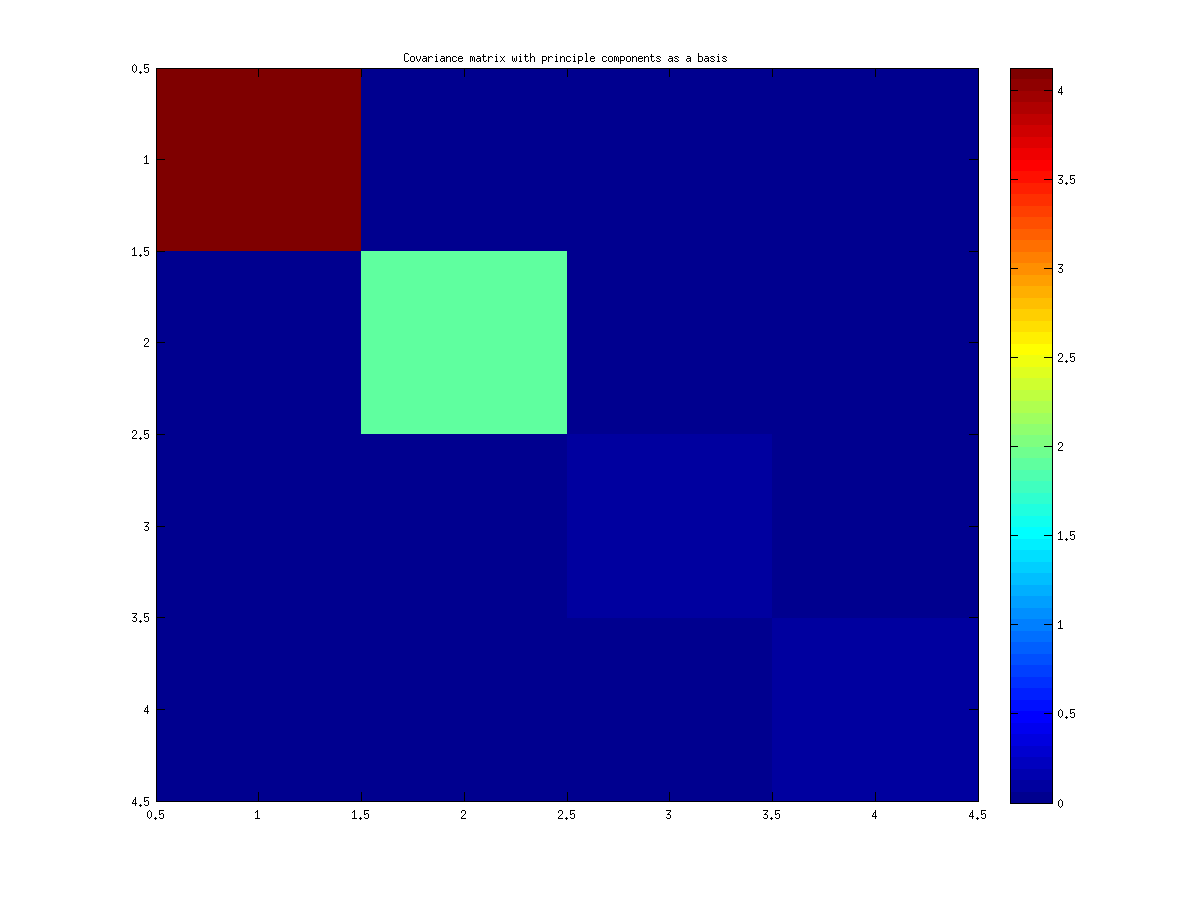
\includegraphics[width=10cm]{task2Eigenvalues.png}
			\caption{Covariance matrix of projected data}
			\label{fig:task2Eigenvalues}
		\end{figure}
		
		\begin{figure}[ht!]
			\centering
			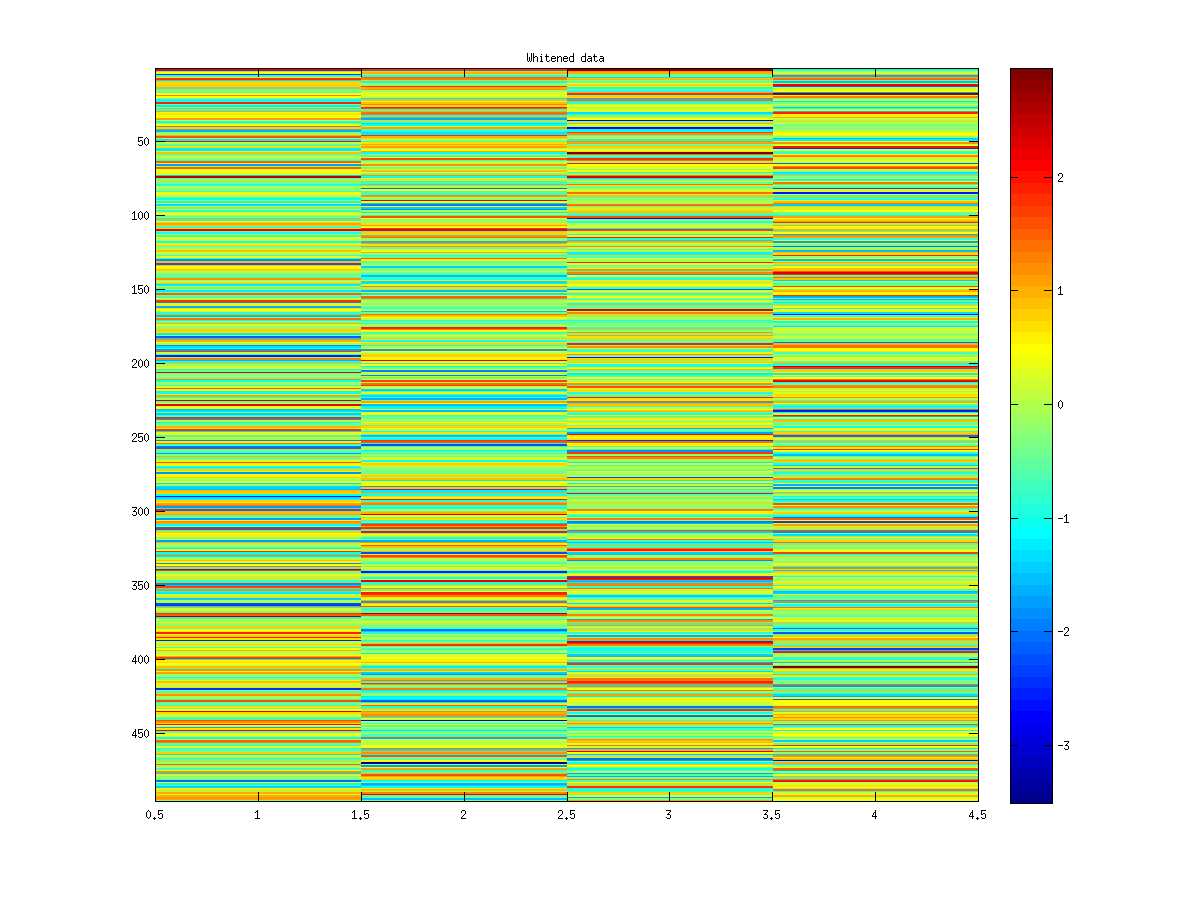
\includegraphics[width=10cm]{task2WhitenedData.png}
			\caption{Whitened data}
			\label{fig:task2WhitenedData}
		\end{figure}
		
	\subsection{Rotation}
		We used the kernel estimator with the hyperparameter $h=0.5$ to estimate the marginal densities.
		\begin{figure}[H]
			\centering
			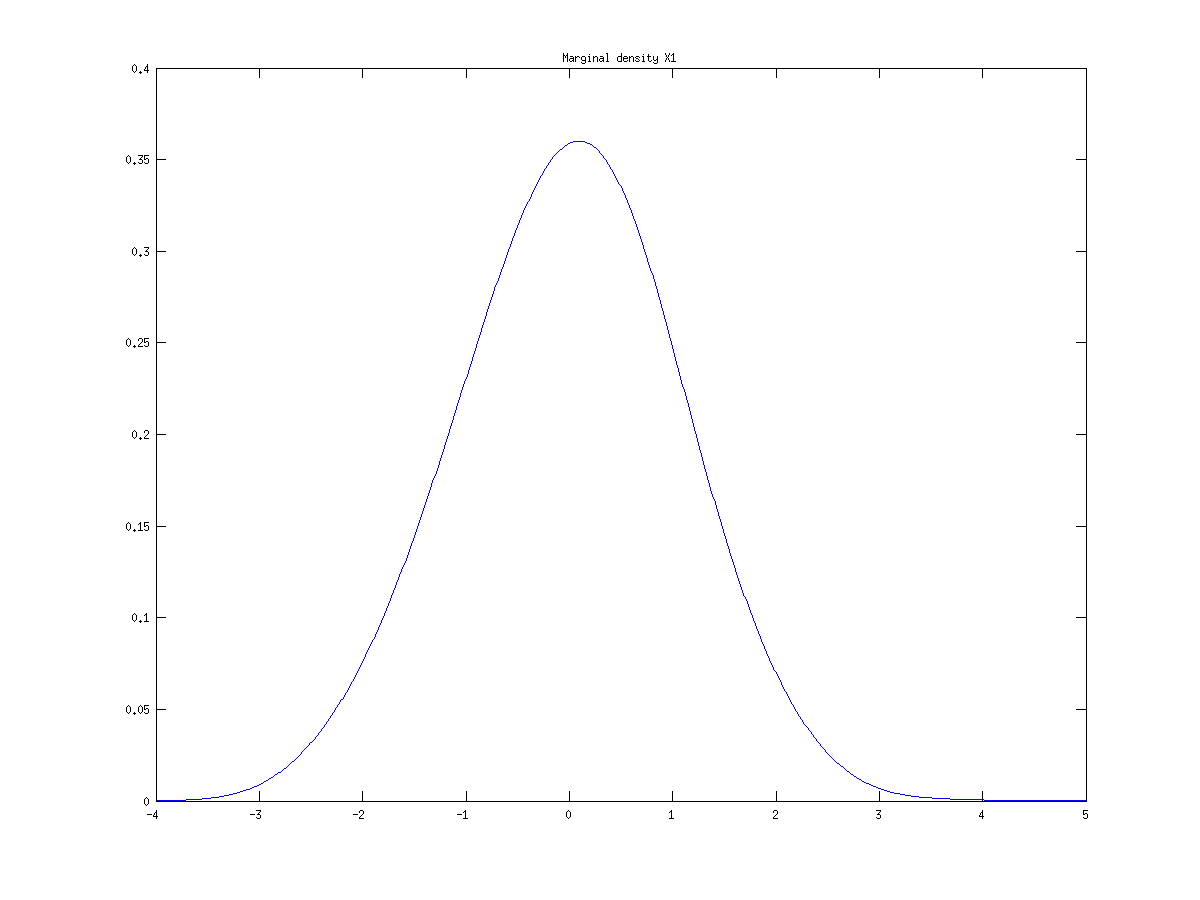
\includegraphics[width=10cm]{task3MarginalDensityX1.png}
			\caption{Marginal density X1}
			\label{fig:task3MarginalDensityX1}
		\end{figure}
		\begin{figure}[H]
			\centering
			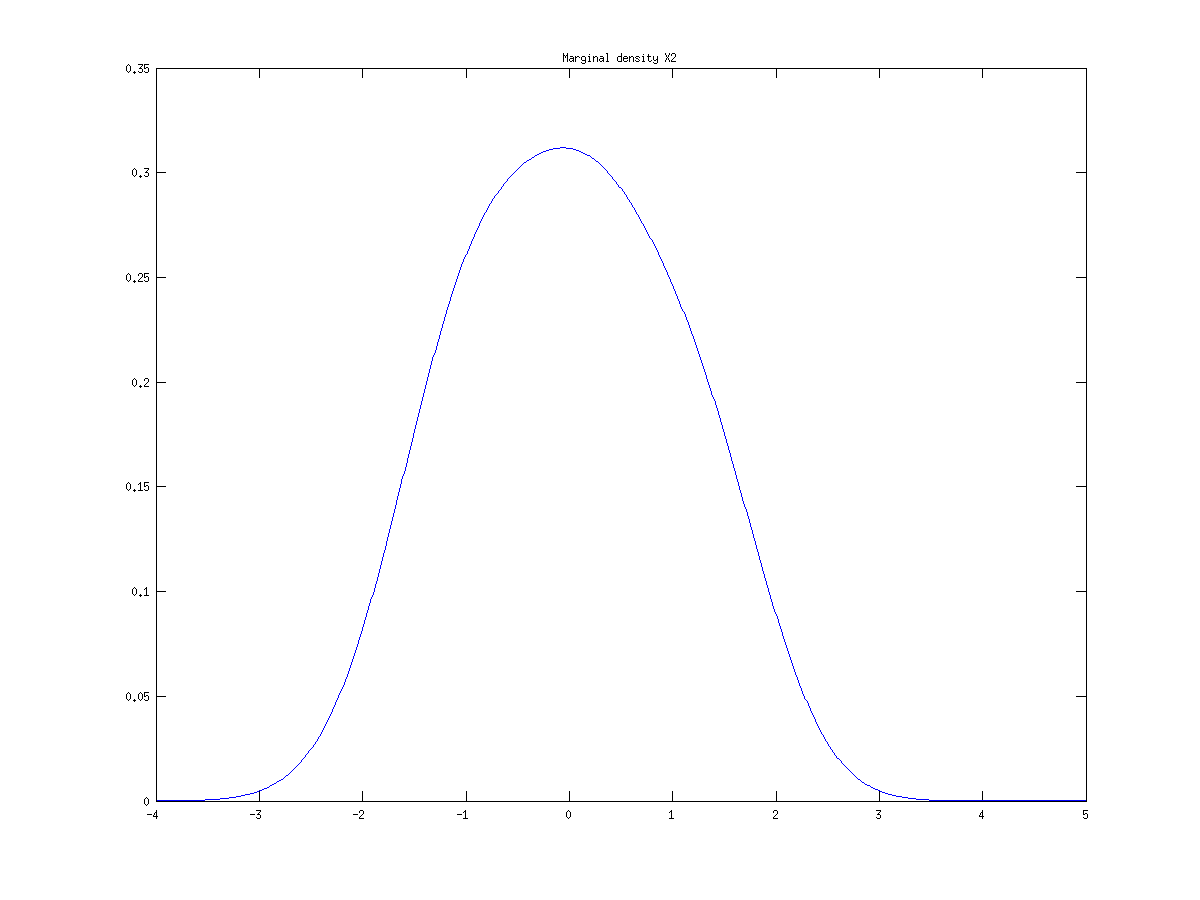
\includegraphics[width=10cm]{task3MarginalDensityX2.png}
			\caption{Marginal density X2}
			\label{fig:task3MarginalDensityX2}
		\end{figure}
		
		The projected data onto the principle components can be found in Figure \ref{fig:task3ProjectedData}.
		\begin{figure}[H]
			\centering
			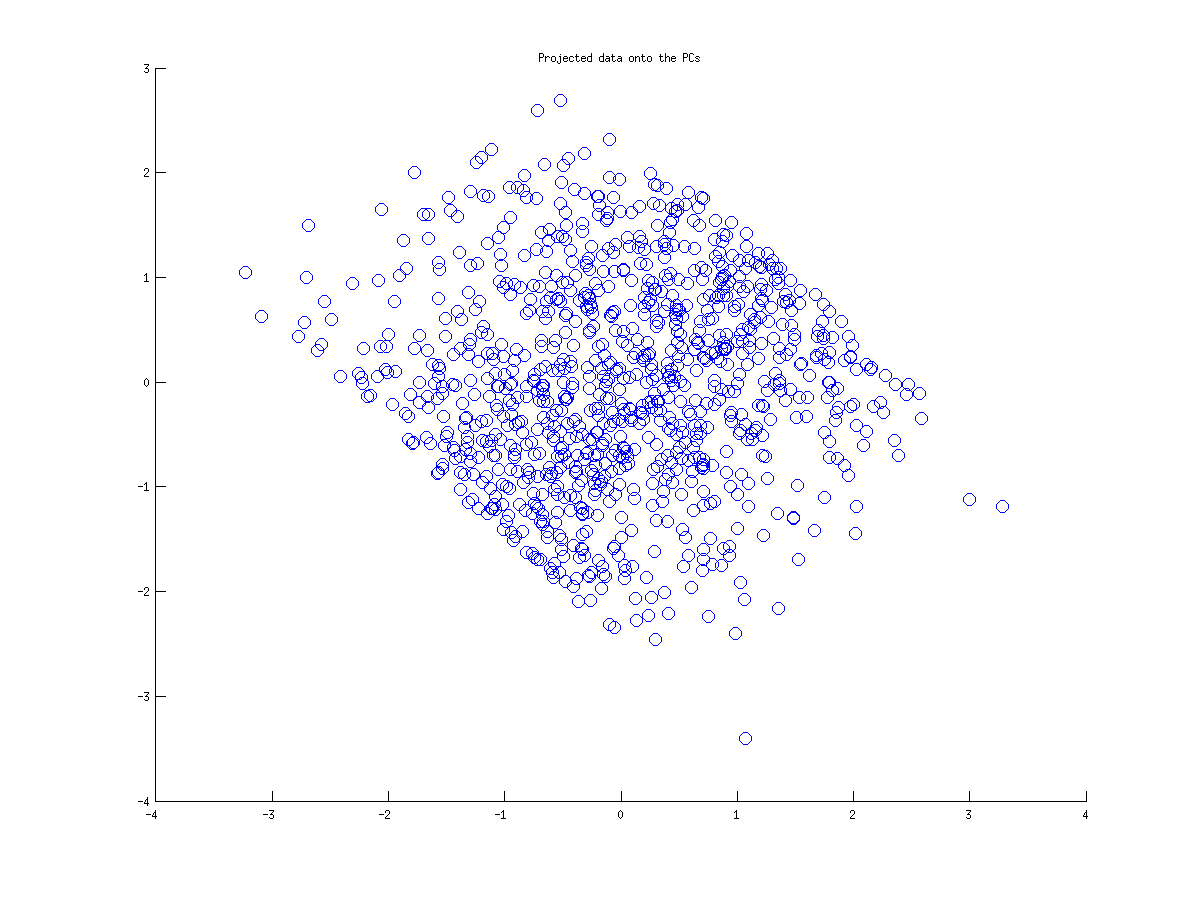
\includegraphics[width=10cm]{task3ScatterProjectedData.png}
			\caption{Plot of projected input data onto principle components}
			\label{fig:task3ProjectedData}
		\end{figure}
		The influence of the whitening, scaling of the data in x and y direction such that the covariance is 1, is illustrated in Figure \ref{fig:task3ProjectedWhitened}.
		\begin{figure}[H]
			\centering
			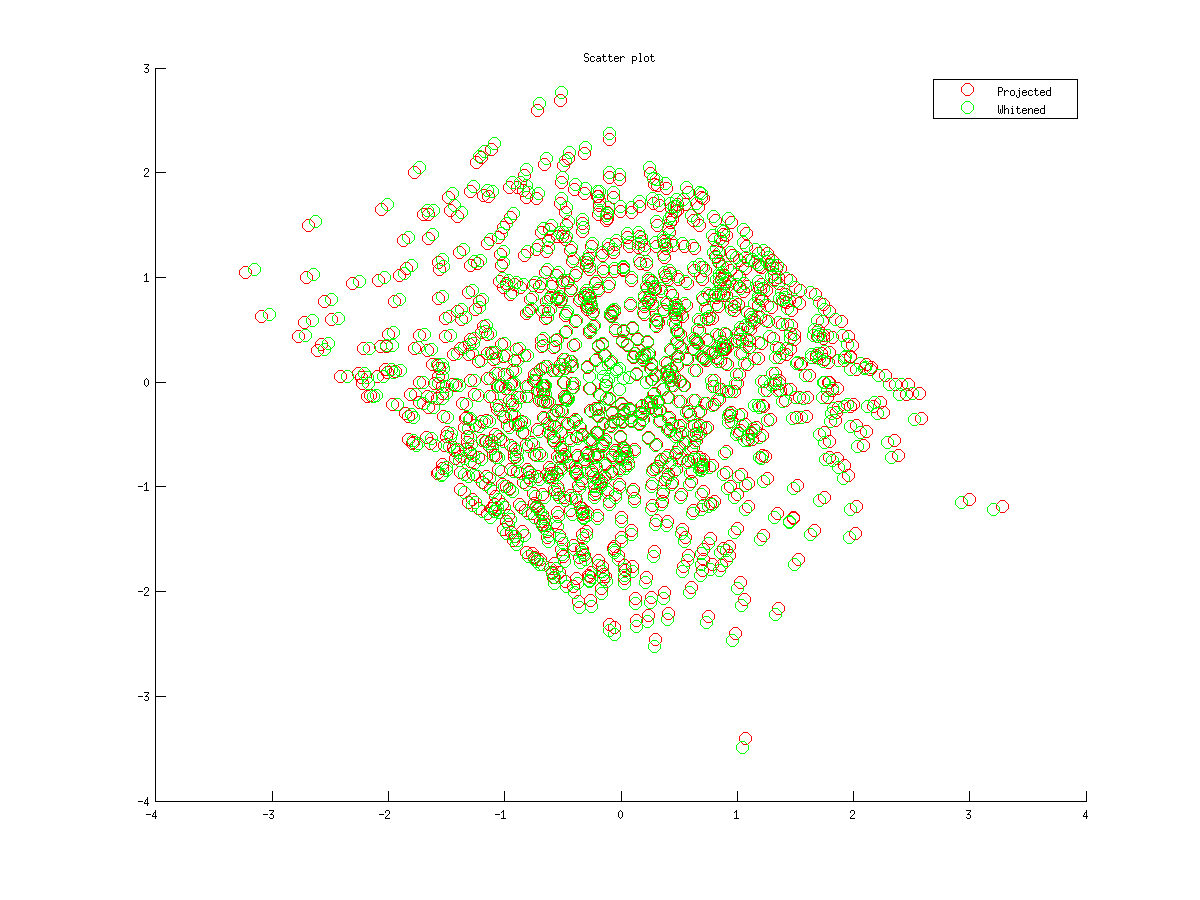
\includegraphics[width=10cm]{task3ScatterPlotProjectedWhitened.png}
			\caption{Plot of projected and whitened data}
			\label{fig:task3ProjectedWhitened}
		\end{figure}
		In the following we have used an angle of $45^{\circ}$ for the rotation.
		The marginal densities of the whitened and the rotated data can be found in Figures \ref{fig:task3MDWRX1} and \ref{fig:task3MDWRX2}.
		\begin{figure}[H]
			\centering
			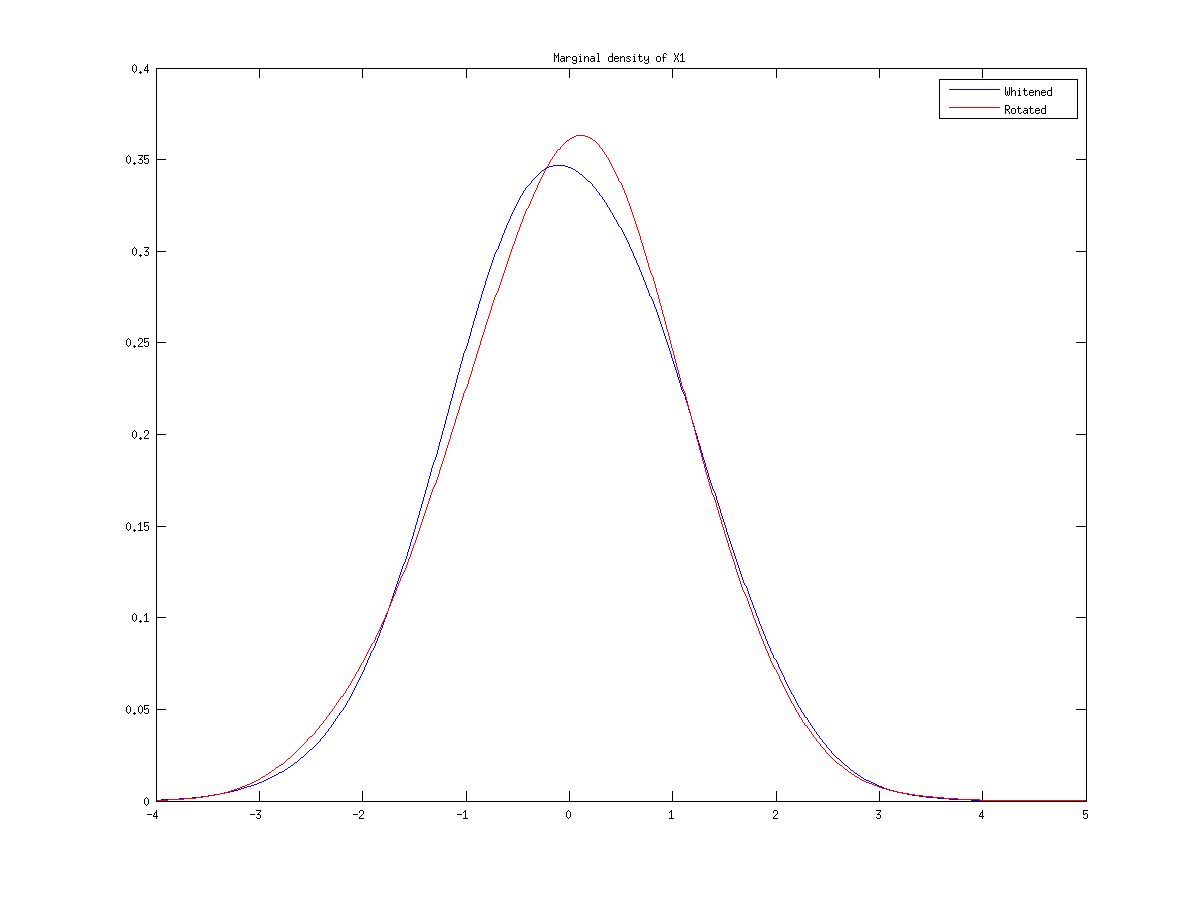
\includegraphics[width=10cm]{task3MarginalDensityX1WhitenedRotated.png}
			\caption{Marginal density of X1, comparison whitened and rotated}
			\label{fig:task3MDWRX1}
		\end{figure}
		
		\begin{figure}[H]
			\centering
			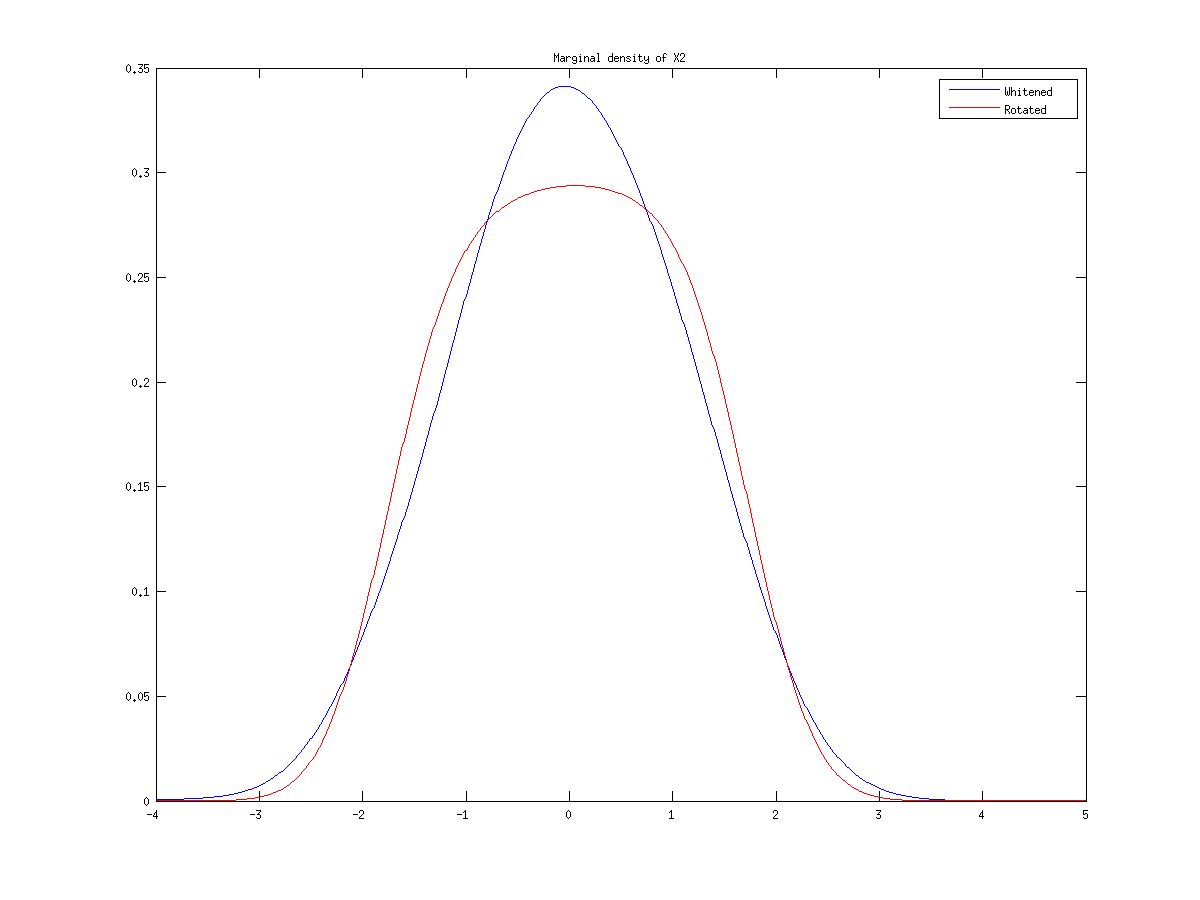
\includegraphics[width=10cm]{task3MarginalDensityX2WhitenedRotated.png}
			\caption{Marginal density of X2, comparison whitened and rotated}
			\label{fig:task3MDWRX2}
		\end{figure}
		
		It can be seen that the marginal densities are dependent on the rotation angle.
		We compare now the covariance matrices. The covariance matrix of the input data is given in Figure \ref{fig:task3Covariance}.
		
		\begin{figure}[H]
			\centering
			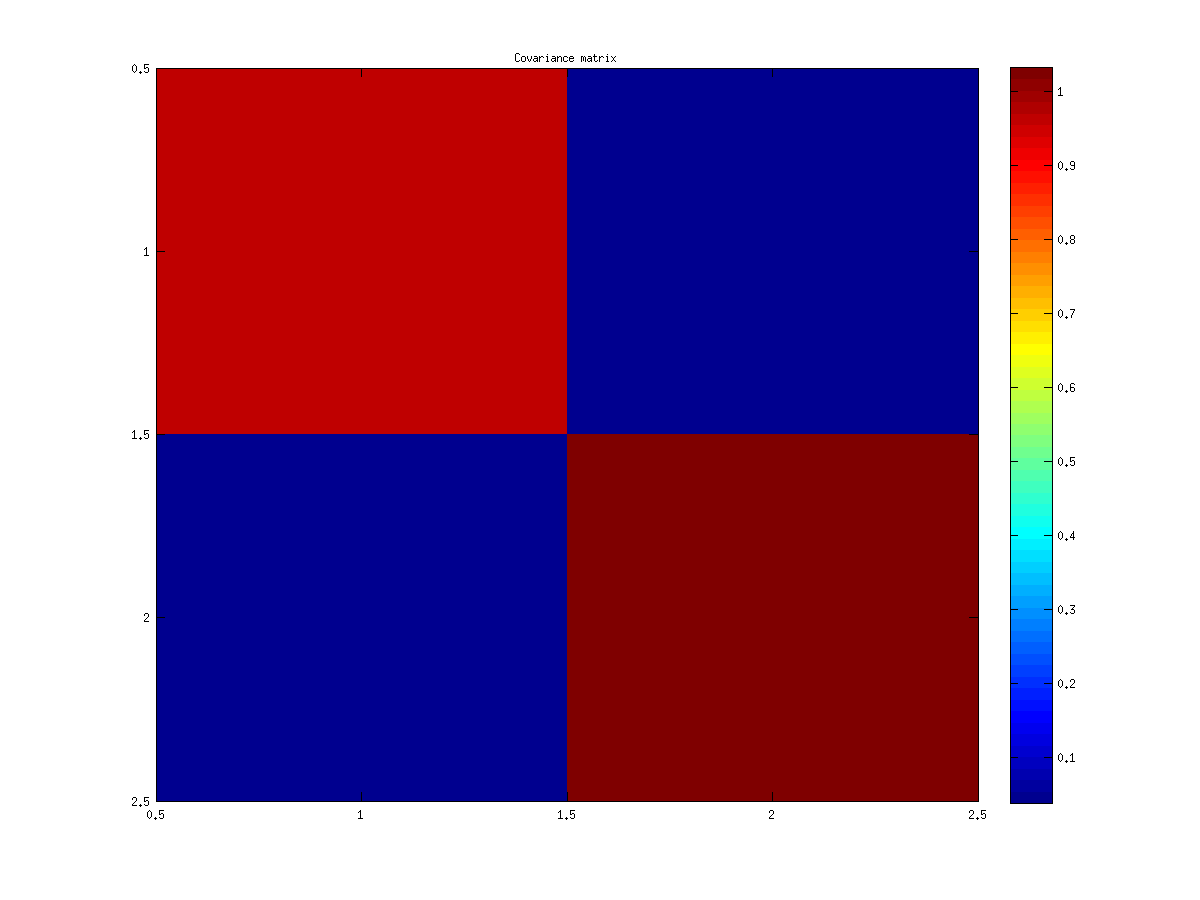
\includegraphics[width=10cm]{task3Covariance.png}
			\caption{Covariance matrix of input data}
			\label{fig:task3Covariance}
		\end{figure}
		
		One can see, that the variances of the diagonal elements are not equal. Moreover, the off-diagonal elements are non-zero. 
		Compared to that we see in Figure \ref{fig:task3CoW} the covariance matrix of the whitened data.
		
		\begin{figure}[H]
			\centering
			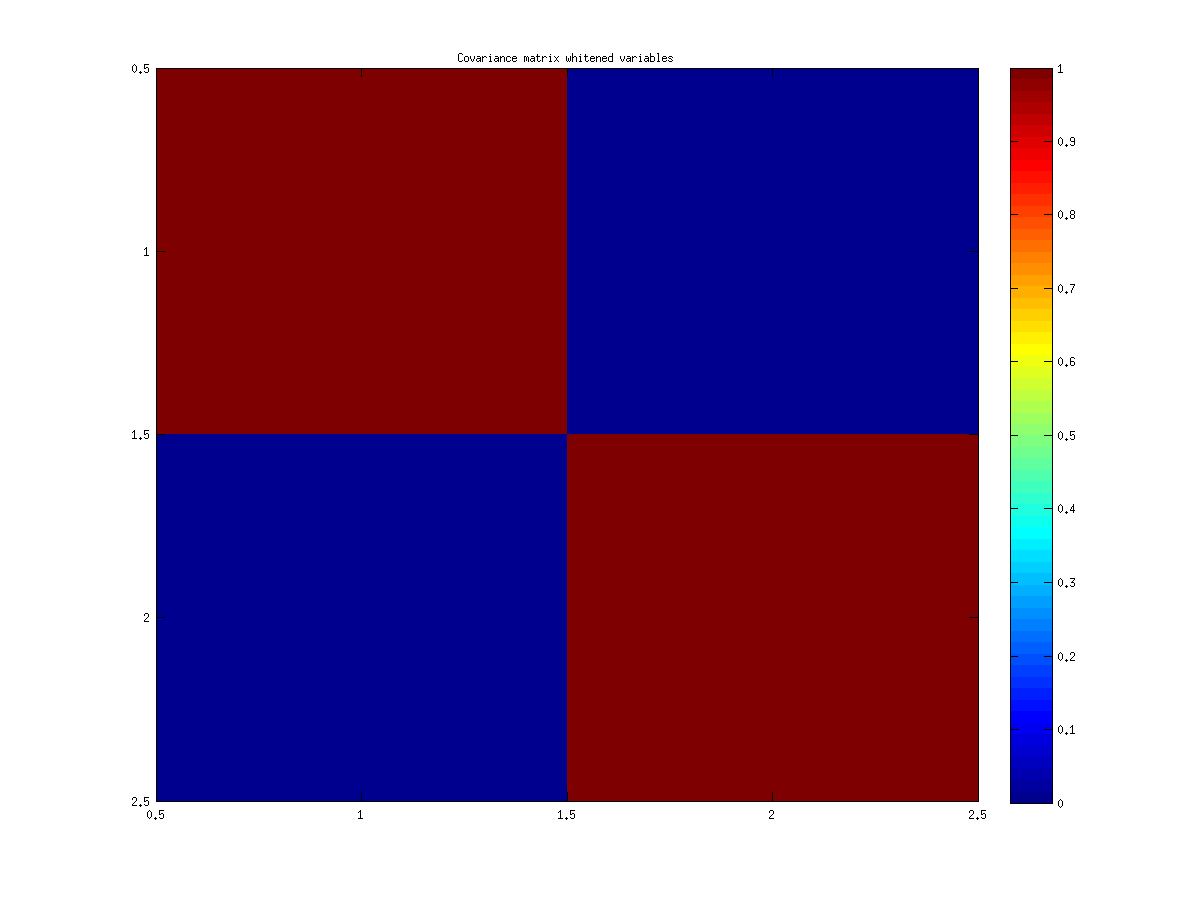
\includegraphics[width=10cm]{task3CovarianceWhitened.png}
			\caption{Covariance matrix of whitened data}
			\label{fig:task3CoW}
		\end{figure}
		
		Here we can see that the covariance matrix of the whitened data is the identity matrix. Moreover, Figure \ref{fig:task3CoWR} shows that the covariance of whitened data is invariant with respect to rotation. This becomes quite clear if one considers that the identity matrix has only the eigenvalue $1$ and the corresponding eigenraum spans $\mathbb{R}^2$.  
		
		\begin{figure}[H]
			\centering
			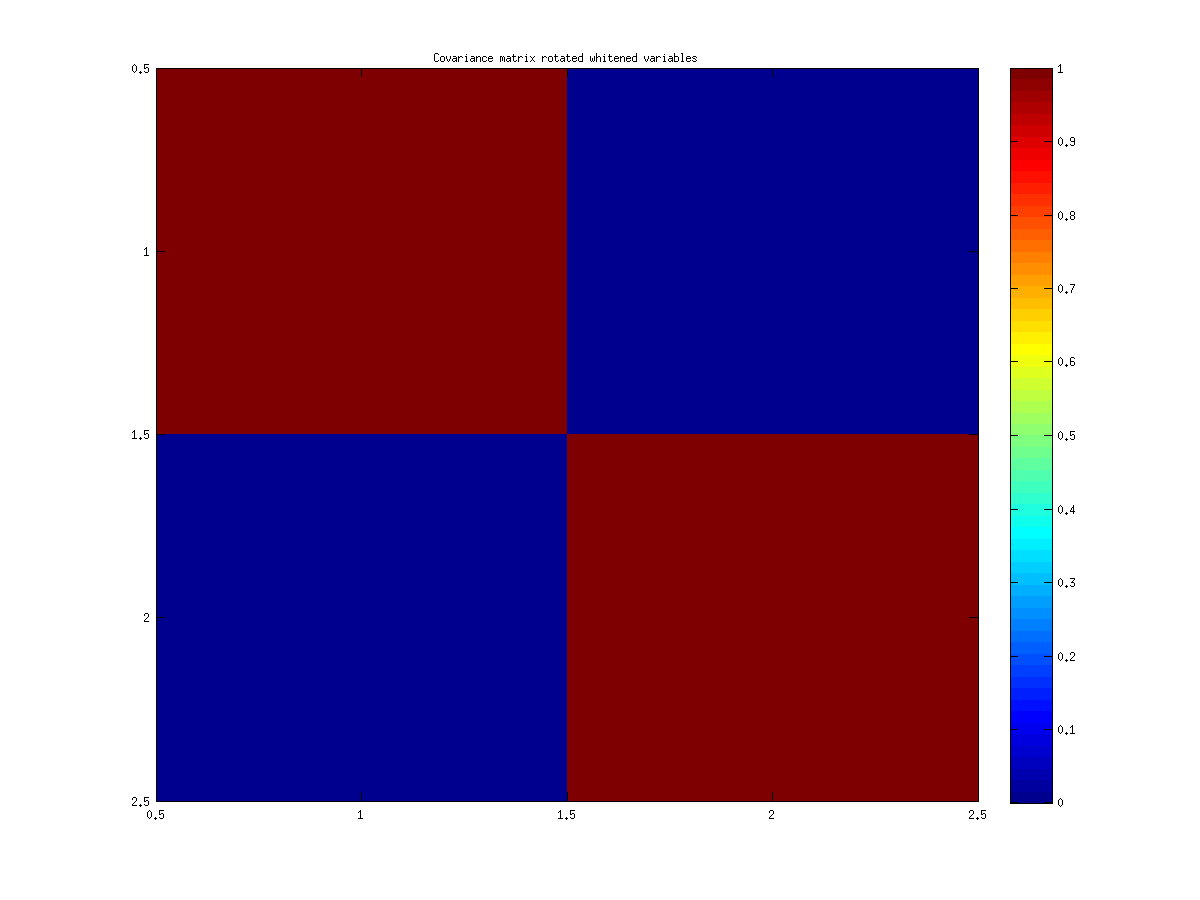
\includegraphics[width=10cm]{task3CovarianceRotated.png}
			\caption{Covariance matrix of whitened and rotated data}
			\label{fig:task3CoWR}
		\end{figure}
		
		Let $\Sigma=I$ be the covariance matrix of the whitened data $Z$ and $Z^{\prime}=(RZ^{T})^{T}$ be the rotated data. Then the corresponding covariance matrix is given by:
		\begin{eqnarray}
			\Sigma^{\prime} &=& (Z^{\prime})^{T}\cdot Z^{\prime}\\
			&=& RZ^{T}\cdot ZR^{T}\\
			&=& R\Sigma R^{T}\\
			&=& I
		\end{eqnarray}
		
\end{document}
